% !TeX root = RJwrapper.tex
\title{\pkg{mistr}: A Computational Framework for Mixture and Composite Distributions}
\author{by Lukas Sablica and Kurt Hornik}

\maketitle

\abstract{%
Finite mixtures and composite distributions allow to model the
probabilistic representation of data with more generality than simple
distributions and are useful to consider in a wide range of
applications. The R package \pkg{mistr} provides an extensible
computational framework for creating, transforming, and evaluating these
models, together with multiple methods for their visualization and
description. In this paper we present the main computational framework
of the package and illustrate its application. In addition, we provide
and show functions for data modeling using two specific composite
distributions as well as a numerical example where a composite
distribution is estimated to describe the log-returns of selected
stocks.
}

% Any extra LaTeX you need in the preamble

\newcommand{\class}[1]{\textmd{\textsl{#1}}}
\newcommand{\fun}[1]{\texttt{#1}}

\hypertarget{introduction}{%
\section{Introduction}\label{introduction}}

During the history of financial mathematics mankind has developed many
useful theories how to describe financial markets.
While the models in asset pricing are generally covered by the 
central limit theorem (CLT) arguments, these arguments do not 
cover the tail behaviour and thus are usually not appropriate in the
risk management with its focus on the tails of the distribution. 
%Some of these
%theories assume that the market behavior can be described using one
%simple distribution. For example, in case of stock log-returns it is
%commonly a bad practice to assume the normal distribution, even if we
%see that the empirical distributions are generally heavy tailed. But can
%these market movements, which represent how we, highly advanced beings,
%think and act, be described by only one standard distribution? The same
%way we think differently in different moods or extreme situations, the
%distribution describing our behavior in these situations can change.
A simple illustration might be the log-returns distribution of the German
multinational software corporation
\href{https://en.wikipedia.org/wiki/SAP_SE}{SAP}. Clearly, the tails are
much heavier than in the case of normal distribution with the same mean
and standard deviation. This behavior can be frequently found in a
number of financial assets.

\begin{Schunk}

\begin{figure}[h]
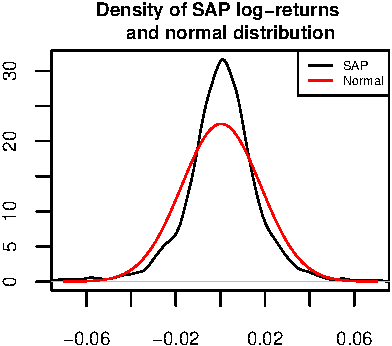
\includegraphics{sablica-hornik_files/figure-latex/unnamed-chunk-1-1} 
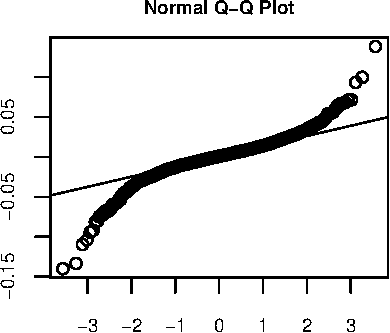
\includegraphics{sablica-hornik_files/figure-latex/unnamed-chunk-1-2}
\caption{Left: Densities of the normal distribution and daily SAP log-returns from January 2007 to October 2017. Right: Quantile-quantile plot of the normal distribution against SAP log-returns.}
\end{figure}
\end{Schunk}

A more interesting result can be seen from the quantile-quantile plot.
While the normal distribution fails in the tails, it excels in the
center. This suggests to use a more suitable distribution which can
catch the fat tails presented above, yet follows a normal distribution
in the center.

A simple answer to this idea is the concept of composite distributions (also known as spliced distributions) and mixture models, where one assumes that the distribution is a finite
mixture of component distributions defined as
\begin{equation} \label{composite}
F(x)=\sum_{i=1}^{n}w_{i}F_{i}\left (x|B_{i}  \right ), \qquad f(x)=\sum_{i=1}^{n}\frac{w_{i}}{F_{i}\left (  B_{i} \right )}1_{B_{i}}\left ( x \right )f_{i}(x)
\end{equation} and \begin{equation} \label{mixture}
F(x)=\sum_{i=1}^{n}w_{i}F_{i}\left (x  \right ), \qquad f(x)=\sum_{i=1}^{n}w_{i}f_{i}\left (x  \right ),
\end{equation} respectively, where \(w_{1},w_{2},\ldots,w_{n}\) are
positive weights that sum up to one, \(B_{1},B_{2}, \ldots ,B_{n}\) are
Borel sets giving a disjoint partition of the support, \(1_{B_{i}}\) is
the indicator function of a set \(B_{i}\), and
\(F_{1},F_{2},\ldots,F_{n}\) are the probability distributions over
\(\mathbb{R}\) with \(F_{i}(B_{i})>0\) for all \(i=1,2,\ldots,n\).
Obviously, the composite models are a specific case of the mixture
models, where the corresponding probability distribution functions are
truncated to some disjoint support. For the presented data, a
three-component composite model with the first and third component being
some heavy-tailed distribution and its negative transform, respectively,
is clearly something that might be appropriate. Note that this also
suggests the need of a transformation framework that would be able to
perform monotonic transformations on the random variables that represent
these exceedance distributions. This innovation is motivated by the fact
that even though most of the extreme value distributions belong to the
location-scale family, without a decreasing transformation these
distributions cannot be used for modeling of heavy left tails.

Moreover, composite models have gained a fair amount of attention in
actuarial loss modeling. Most frequently one employs models composed of
two components, where the first is based on the log-normal distribution
and defined on the positive reals, and the second distribution is chosen
according to the data set to model extreme measurements. Common choices
for these tail-modeling distributions are, for instance, the generalized
Pareto distribution or the Burr distribution. Such models have been
proposed by various authors, for more details see \citet{2b}, \citet{3c}
and \citet{5}.

To offer a general framework for univariate distributions and for
mixtures in general, package \CRANpkg{mistr} is specifically designed to
create such models, evaluate or even fit them. This article introduces
\pkg{mistr} and illustrates with several examples how these
distributions can be created and used.

\hypertarget{distributions-in-r}{%
\section{Distributions in R}\label{distributions-in-r}}

\begin{wrapfigure}{r}{0.2\textwidth}
    \centering
    
\includegraphics[width=0.2\textwidth]{sablica-hornik_files/sticker.png}
\end{wrapfigure}

R currently employs the naming convention {[}prefix{]}{[}name{]}, where
{[}name{]} corresponds to the name of the desired distribution and
{[}prefix{]} is one of `p', `d', `q' or `r', indicating, respectively,
the distribution, density and quantile functions, or random number
generation. However, there are many of restrictions in this concept.
What would be desirable is that one would be able to treat a
distribution as a variable and so to be able to send it to a function or
perform transformations on the random variable it represents.

Naturally, one way to do this is by using the object oriented system in
R. To even improve this idea, one can use some favored dispatching
mechanism, like S3 or S4, to let the computer decide how to handle the
corresponding distribution correctly and which functions to use. In
particular, the prefixes p, d, q, and r can still be just smartly
evaluated as generic functions with appropriate methods. Moreover, with
such a system we can add other useful calls and so take the distribution
operations to the next level, such as monotonic transformation of a
distribution. Additionally, once these objects containing all necessary
information about the distributions are defined, they can be then reused
for the purpose of the mixture and composite distributions.

This approach has already been used in the package \CRANpkg{distr}
\citep{7}, which provides a conceptual treatment of distributions by
means of S4 classes. A parent class \textmd{\textsl{Distribution}}
allows to create objects and contains a slot for parameters as well as
for the four methods mentioned above, \texttt{p()}, \texttt{d()},
\texttt{q()}, and \texttt{r()}. While \pkg{distr} provides several
classes for distributions and finite mixtures in general, like
many similar packages, to the best of our knowledge it does not
%support any tools to work with composite distributions
contain any generating functions for the composite distributions.
In particular, the only packages available for composite
models are  \CRANpkg{CompLognormal} \citep{2b}, \CRANpkg{evmix} \citep{evmix}, \CRANpkg{OpVar} \citep{OpVaR}, \CRANpkg{ReIns}  \citep{ReIns} and \CRANpkg{gendist} \citep{gendist}, which do not offer a general framework for composite models with more than two components. Whereas \pkg{distr} provides an
impressive functionality-rich and extensible framework implemented in
S4, we decided after careful deliberation to realize \pkg{mistr} based
on a self-contained, light-weight framework using S3. This offers to
adjust the representations and settings of the distributions exactly to
the required needs by either mixture or composite models.

The framework provided by package \pkg{mistr} currently supports all
distributions that are included in the \pkg{stats} package and, in
addition, it offers some extreme value distributions like generalized
Pareto, Pareto, Frechet, and Burr. In case that the user would like to
use a distribution that is not directly supported by the framework, a
new distribution can be implemented in a very simple way. This procedure
is documented in detail in the
\href{https://cran.r-project.org/web/packages/mistr/vignettes/mistr-extensions.pdf}{Extensions vignette}
of the package.

As was already mentioned, the objects in R that represent a distribution
need to contain all the necessary information. This is, of course, for
the purpose of evaluating the distribution function or quantile function
at suitable points just the knowledge of the parameters. Since the
framework we propose is beyond a simple distribution evaluation, the
representation is a little bit more complex. A simple random variable or
a distribution is in our framework represented by the distribution
family which the distribution follows, together with the proper
parameters and some additional information that corresponds to the
distribution. This information is either stored as a type of class or as
attributes in a list. The framework then uses the S3 dispatching
mechanism to use this information, and hence it works with the
distribution. Such a representation allows to go beyond the simple p, d,
q, and r evaluation and enables to define new and more complicated
functions.

An example is the left-hand limit of the cumulative distribution
function. It might not look of crucial importance to be able to evaluate
\(F(x-)=\mathbb{P}(X<x)\), but this function plays a huge role in the
transformations and composite distributions. Of course, this function
differs from the standard distribution function only if it is applied to
a distribution with a positive probability mass in the point of
interest. For this reason we simply characterize the (``pseudo'')
support by the three parameters ``from'', ``to'' and ``by''. While the
parameters ``from'' and ``to'' specify the range in which the
distribution takes positive values, the parameter ``by'', which is only
a part of the lattice-valued distributions, describes the deterministic
step in the support and for most known discrete distributions is equal
to one, since they have support just on the integers. It might of course
differ for some distributions, which have support only on even numbers,
or some scaled distributions. It is essential that this parametrization
allows to perfectly define the support of a distribution, and hence
allows to do more complicated operations and calculations, e.g., the
left-hand limit of the distribution function. In the case the user would
like a distribution with no equally distanced outcomes, one can perform
a non-linear transformation, which will be dealt with in the next
chapter.

\hypertarget{combining-distributions}{%
\subsection{Combining distributions}\label{combining-distributions}}

Having the framework defined for the simple distributions, it is desired
to combine these objects in order to define a larger class of
distributions. The framework currently supports the mixture and
composite models given in, respectively, \eqref{mixture} and
\eqref{composite}.

Following the definition of the composite models in the univariate case,
the interval representation of the truncation allows to use a sequence
of breakpoints
\[-\infty=\beta_{0}<\beta_{1}\leq\beta_{2}\leq \dots \leq \beta_{n-1}<\beta_{n}=\infty\]
to fully characterize the partitions \(B_{1},B_{2}, \ldots ,B_{n}\).
Note that if \(F_{i}\) is continuous, to ensure that the interval has
positive probability we must take \(\beta_{i-1}<\beta_{i}\).

This allows to define \(\lambda_1=0\) and for all \(i=2,\ldots,n,\)
\[ \lambda _{i}=\left\{\begin{matrix}
F_{i}(\beta_{i-1})  & \text{if } \beta_{i-1}\notin B_{i},  \\ 
F_{i}(\beta_{i-1^{}}-)  & \text{otherwise},
\end{matrix}\right.\] where as before \(F_{i}(\beta_{i-1^{}}-)\) is the
left-hand limit \(\mathbb{P}(X_{i}<x)\), and for all
\(i=1,2,\ldots,n-1,\) \[
\rho _{i}=\left\{\begin{matrix}
F_{i}(\beta_{i})  & \text{if }  \beta_{i}\in B_{i},  \\ 
F_{i}(\beta_{i^{-}}) & \text{otherwise},
\end{matrix}\right.
\] with \(\rho_{n}=1\). Then for any \(x \in B_{i}\) \[
F_{i}\left ( \left (  -\infty,x  \right ] \cap B_{i} \right )=\left\{\begin{matrix}
  F_{i}\left ( x  \right )-  F_{i}\left ( \beta_{i-1}  \right )  & \text{if }  \beta_{i-1}\notin B_{i},\\ 
  F_{i}\left ( x  \right )-  F_{i}\left ( \beta_{i-1}  -\right )  & \text{if }  \beta_{i-1}\in B_{i}.
\end{matrix}\right. 
\] This means that for every \(x \in B_{i}\) we can write the
distribution as
\(F_{i}\left ( \left ( -\infty,x \right ] \cap B_{i} \right )=F_{i}\left ( x \right )-\lambda _{i}\).

The straightforward implication of the above equations is that
\(\sup_{x\in B_{i}}F_{i}\left ( x \right )=\rho _{i}\). Thus, \[
F_{i}\left ( B_{i} \right )=\rho _{i}-\lambda_{i}.
\] Hence, if we define \(p_{i}=\sum_{j:j\leq i}w_{i}\) the composite
distribution satisfies \[
F(x)=p_{i-1}+w_{i}\frac{F_{i}(x)-\lambda_{i}}{F_{i}(B_{i})}=p_{i-1}+w_{i}\frac{F_{i}(x)-\lambda_{i}}{\rho_{i}-\lambda_{i}}, \quad \forall x\in B_{i}
\] and, in addition, \[
p_{i-1}\leq F(x)\leq p_{i} , \quad \forall x\in B_{i} \quad \text{and} \quad \sup_{x\in B_{i}}F(x)=p_{i}.
\]

If we take some \(p \in (0,1)\), then since \(\sum_{i}p_{i}=1\), there
exists \(i\) such that \(p_{i-1}<p<p_{i}\) or \(p=p_{i}\). From this it
follows that

\[
F(x)\geq p \Leftrightarrow F_{i}(x)\geq \lambda_{i}+\frac{p-p_{i}}{w_{i}}\left ( \rho_{i}-\lambda_{i} \right ),
\] which implies \[
F^{-1}(p)=F^{-1}_{i} \left (\lambda_{i}+\frac{p-p_{i}}{w_{i}}\left ( \rho_{i}-\lambda_{i} \right )  \right ), \quad \text{for } p_{i-1}<p\leq p_{i}.
\] Using the quantile transformation method and the above quantile
function we can easily simulate from our composite distribution.

Therefore, to fully specify a composite distribution, in addition to the
mixture specifications, one needs to set the values that correspond to
the breakpoints, which split \(\mathbb{R}\) into disjoint partitions.
Moreover, if at least one distribution is not absolutely continuous, it
might be desired to specify to which adjacent interval should the
breakpoint be included.

\hypertarget{computational-framework}{%
\section{Computational framework}\label{computational-framework}}

The objects representing a simple distribution can be created very
easily. The creator functions follow a standard naming convention from R
where the ``dist'' suffix is appended to the name of a distribution, and
the parameters are entered as arguments. Thus, an object representing
normal distribution with mean equal to 1 and standard deviation equal to
3 can be created as follows:

\begin{Schunk}
\begin{Sinput}
N <- normdist(mean = 1, sd = 3)
N
\end{Sinput}
\begin{Soutput}
#>  Distribution       Parameters
#>     Normal    mean = 1, sd = 3
\end{Soutput}
\end{Schunk}

Once the objects are created, they can be used for evaluation of various
functions. The most commonly employed functions clearly will be the
methods for \texttt{print()} already demonstrated, and the methods for
the functions \texttt{p()}, \texttt{d()}, \texttt{q()} and \texttt{r()}.
These can be easily evaluated as

\begin{Schunk}
\begin{Sinput}
d(N, c(1, 2, 3))
\end{Sinput}
\begin{Soutput}
#> [1] 0.1329808 0.1257944 0.1064827
\end{Soutput}
\begin{Sinput}
p(N, c(1, 2, 3))
\end{Sinput}
\begin{Soutput}
#> [1] 0.5000000 0.6305587 0.7475075
\end{Soutput}
\begin{Sinput}
q(N, c(0.1, 0.2, 0.3))
\end{Sinput}
\begin{Soutput}
#> [1] -2.8446547 -1.5248637 -0.5732015
\end{Soutput}
\begin{Sinput}
r(N, 3)
\end{Sinput}
\begin{Soutput}
#> [1]  1.8144430 -2.6908086  0.2704776
\end{Soutput}
\end{Schunk}

Additional important functions provided by \pkg{mistr} are
\texttt{plim()} and \texttt{qlim()}, which implement, respectively, the
already mentioned left-hand limit of the cumulative distribution
function \(F(x-)=\mathbb{P}(X<x)\) and its pseudoinverse
\[Q(p+) = \inf\left \{ x\in\mathbb{R}: p <  \mathbb{P}\left (X \leq x  \right ) \right \}.\]
Note that the function \texttt{qlim()} plays a very important role when
dealing with the transformations, and just as \texttt{plim()}, in the
case of continuous distributions it simplifies to \texttt{q()}. Clearly
if \(-X\) has a positive probability mass at \(x\), then \[
q=P(-X \leq x)= 1-P(X < -x) \Rightarrow -Q_{X}(1-q+)=x.
\]

\begin{Schunk}
\begin{Sinput}
B <- binomdist(size = 12, prob = 0.3)
plim(B, c(-3, 0, 3, 12))
\end{Sinput}
\begin{Soutput}
#> [1] 0.0000000 0.0000000 0.2528153 0.9999995
\end{Soutput}
\begin{Sinput}
qlim(B, plim(B, c(0, 3, 7, 12)))
\end{Sinput}
\begin{Soutput}
#> [1]  0  3  7 12
\end{Soutput}
\end{Schunk}

\hypertarget{adding-transformation}{%
\subsection{Adding transformation}\label{adding-transformation}}

Once the objects that represent a single distribution are created, we
can use this representation to go beyond the scope of a simple
distribution function evaluation. The knowledge of the distributions
class and support range that is stored inside the object opens the doors
for more complicated operations. One such an operation is the ability to
perform monotone transformations of random variables.

The transformation framework currently allows for all standard monotone
transformations like addition, subtraction, multiplication, division,
logarithm, exponential and monotonic power transformations, where in case 
of binary operators a numeric value must be used as the second operand. Moreover, it is
provided with the knowledge of invariant and direct transformations that
correspond to the distributions it offers. This information is stored as
a generic function that directly dispatches on the class of distribution
family and not on the class \textmd{\textsl{univdist}} to prevent losing
any information about the distribution. An example might be the
exponential distribution where a multiplication with a positive scalar
rather keeps the family and changes the parameters. On the other hand, a
positive power transformation will directly create a Weibull
distribution with appropriate parameters.

\begin{Schunk}
\begin{Sinput}
E <- expdist(2)

E * 2
\end{Sinput}
\begin{Soutput}
#>  Distribution   Parameters
#>  Exponential    rate = 1
\end{Soutput}
\begin{Sinput}
E^2
\end{Sinput}
\begin{Soutput}
#>  Distribution                Parameters
#>    Weibull    shape = 0.5, scale = 0.25
\end{Soutput}
\end{Schunk}

If the transformation is necessary and continuous on the support of the distribution, the transformation dispatches on the
class \textmd{\textsl{univdist}}. For any untransformed distribution,
this function will change the whole class and the class of the
distribution family is removed since the random variable does not follow
the distribution anymore. However, the information is stored for the
case the distribution would need to untransform itself later. The
function then builds an expression for the transformation and inverse
transformation, along with a print expression and an expression for the
derivative of the inverse transformation. Besides these list members,
also a history member is stored, a list that records the information
about the old transformations and becomes really handy when it comes to
an inverse transformation of the previous one, or updating a
transformation. A simple example of a transformation and update follows.

\begin{Schunk}
\begin{Sinput}
E2 <- E * -2
E3 <- E2 * 5
E3
\end{Sinput}
\begin{Soutput}
#>    Trafo Distribution Parameters
#>  -10 * X  Exponential   rate = 2
\end{Soutput}
\end{Schunk}

The next example uses the normal distribution that we created in the
last chapter.

\begin{Schunk}
\begin{Sinput}
Norm_trafo <- (N - 1)^(1/3)
Norm_trafo
\end{Sinput}
\begin{Soutput}
#>    Trafo Distribution       Parameters
#>  X^(1/3)       Normal mean = 0, sd = 3
\end{Soutput}
\end{Schunk}

\noindent Note that the \(X-1\) transformation is not displayed in the
Trafo column as it is an invariant transformation that rather changed
the parameter mean from 1 to 0.

The methods that evaluate the transformed distribution are called in the
same fashion as the non-transformed distributions. Additionally, the new
pseudo description of the support can be returned using
\texttt{sudo\textunderscore support()}, which gives two numeric values
(``From'' and ``To'') describing the range of the support.

\begin{Schunk}
\begin{Sinput}
Binom_trafo <- -3 * log(B + 4)

q(Binom_trafo, c(0.05, 0.5, 0.95))
\end{Sinput}
\begin{Soutput}
#> [1] -6.907755 -6.238325 -4.828314
\end{Soutput}
\begin{Sinput}
plim(Binom_trafo, c(-6, -5, 0))
\end{Sinput}
\begin{Soutput}
#> [1] 0.5074842 0.9149750 1.0000000
\end{Soutput}
\begin{Sinput}
sudo_support(Binom_trafo)
\end{Sinput}
\begin{Soutput}
#>      From        To 
#> -8.317766 -4.158883
\end{Soutput}
\end{Schunk}

\subsection{Visualization}

In addition, the \texttt{plot()} and \texttt{autoplot()} generics can be
called. These methods are offered for any distribution object in the
\pkg{mistr} package and return the plot of PDF or PMF and CDF of a given
object. The function uses the introduced \texttt{d()} and \texttt{p()}
functions to evaluate the required values. While the \texttt{plot()}
methods offer a plot constructed using base plotting, the
\texttt{autoplot()} offers an alternative plot that is created using the
\CRANpkg{ggplot2} package \citep{ggplot2}.

\begin{Schunk}
\begin{Sinput}
par(mai = c(0.4, 0.4, 0.2, 0.2))
plot(Norm_trafo, xlim1 = c(-2.5, 2.5), ylab1 = "", cex.axis = 0.75)
\end{Sinput}

\begin{figure}[h]
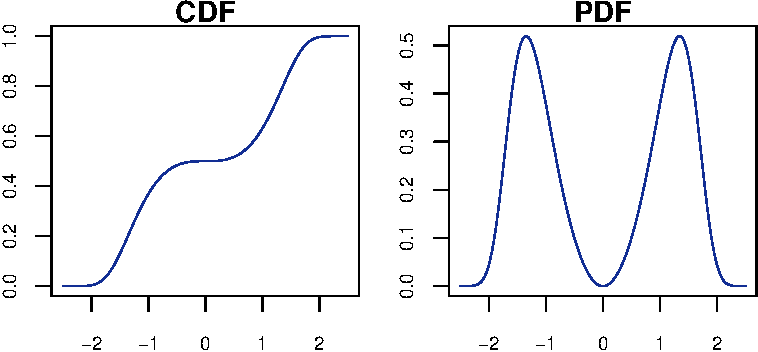
\includegraphics{sablica-hornik_files/figure-latex/unnamed-chunk-9-1}
\caption{CDF (left) and PDF (right) plot of the \texttt{Norm\_trafo} object using \texttt{plot()}.}
\end{figure}
\end{Schunk}

\begin{Schunk}
\begin{Sinput}
library(ggplot2)
autoplot(Norm_trafo, xlim1 = c(-2.5, 2.5))
\end{Sinput}

\begin{figure}[h]
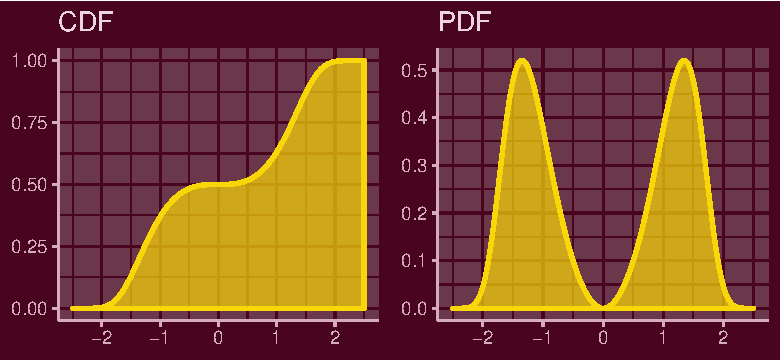
\includegraphics{sablica-hornik_files/figure-latex/unnamed-chunk-10-1} 
\caption{CDF (left) and PDF (right) plot of the \texttt{Norm\_trafo} object using \texttt{autoplot()}.}
\end{figure}
\end{Schunk}


Other plot functions offered for the \pkg{mistr} distribution objects
are \texttt{QQplot()} and \texttt{QQplotgg()}. The methods for this
functions graphically compare the empirical quantiles of two data sets,
or quantiles of two distribution objects, or quantiles of a distribution
with the empirical quantiles of a sample. If quantiles of a continuous
distribution are compared with a sample, a pointwise asymptotic confidence bound for this
data is offered. This confidence ``envelope'' is based on the asymptotic
results of the order statistics. For a distribution \(F\) as the number of observations \(n\) tends
to infinity, the \(p^{th}\) sample quantile is asymptotically
distributed as
\[X_{\left (\left [ np \right ]  \right )} \sim AN\left ( F^{-1}\left ( p \right ),\frac{p(1-p)}{n\left [ f\left ( F^{-1}\left ( p \right ) \right ) \right ]^{2}} \right ),\]
where \(f(x)\) and \(F^{-1}(p)\) are the density function and quantile
function associated with \(F(x)\), respectively. More details can be
found on the
\href{https://en.wikipedia.org/wiki/Order_statistic}{order statistics Wikipedia page}
or in \cite{wilks}, for example. For alternative bounds see \cite{ggqq}.

\begin{Schunk}
\begin{Sinput}
QQplotgg(Norm_trafo, r(Norm_trafo, 1000), conf = 0.99, ylab = NULL, xlab = NULL)
\end{Sinput}

\begin{figure}[h]
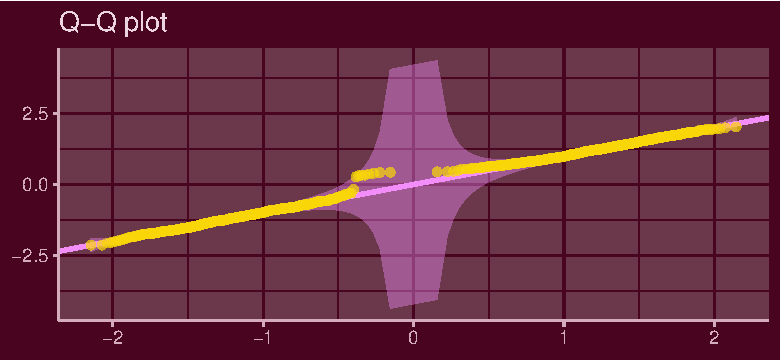
\includegraphics{sablica-hornik_files/figure-latex/unnamed-chunk-11-1}
\caption{Q-Q plot of the \texttt{Norm\_trafo} object against normally distributed sample with 99\% confidence bound.}
\end{figure}
\end{Schunk}
 

\hypertarget{combining-objects}{%
\subsection{Combining objects}\label{combining-objects}}

\hypertarget{mixtures}{%
\subsubsection{Mixtures}\label{mixtures}}

Mixture distributions are fully specified by the components \(F_{i}(x)\)
(i.e., the distributions) and by the weights \(w_{i}\) that correspond
to these components. Function \texttt{mixdist()} allows to create
mixtures by specifying these characterizations. This can be done in two
ways. First, the user may specify the distribution names (names from
{[}prefix{]}{[}name{]} functions), the list of appropriate parameters of
these distributions, and a sequence of weights. An example of such a
call follows.

\begin{Schunk}
\begin{Sinput}
mixdist(c("norm", "unif"), list(c(2, 2), c(1, 5)), weights = c(0.5, 0.5))
\end{Sinput}
\begin{Soutput}
#> Mixture distribution with: 
#>  
#>   Distribution       Parameters       Weight
#> 1    Normal    mean = 2, sd = 2          0.5
#> 2   Uniform    min = 1, max = 5          0.5
\end{Soutput}
\end{Schunk}

Another way is to use the objects that have already been defined. Since
the parameters are already stored inside the object, all the function
requires are the objects and the weights. This also allows to use
transformed distributions from the last chapter or more complicated
objects, which will be presented later. This means that the transformed
normal and binomial distributions together with an exponential
distribution can be reused for mixture distribution as:

\begin{Schunk}
\begin{Sinput}
M <- mixdist(Norm_trafo, Binom_trafo, expdist(0.5), weights = c(0.4, 0.2, 0.4))
\end{Sinput}
\end{Schunk}

The information about the mixture can be accessed via multiple S3
methods. The components can be extracted using square brackets
\texttt{[]}, the weights can be obtained using \texttt{weights()}, and
just as with standard distributions, the parameters are obtainable using
\texttt{parameters()}.

Other interesting methods are those for \texttt{q} and \texttt{qlim} and
\textmd{\textsl{mixdist}} objects. While finding the CDF and PDF of the
mixture model is straightforward, an explicit general expression for
quantile function of the mixture model is not available. However, it can
be found numerically as a solution of a unit-root problem:
\[\sum_{i=1}^{n}w_{i}F_{i}\left (Q(p)  \right )-p=0 .\] What is more,
one can show that the quantile of a mixture distribution \(Q(p)\) can
always be found within the range of its components quantiles, and hence
\[ \min_{i\in\left \{ 1,\dots, n \right \}}Q_{i}(p)\leq Q(p)\leq \max_{i\in\left \{ 1,\dots, n \right \}}Q_{i}(p),\]
where \(Q_{i}(\cdot)\) is the quantile function of the i-th component.
This specifies the needed interval for the root finder that will then
iteratively find the solution. Additionally, further problems are solved
to return the correct values. To show how this algorithm works we
perform a simple test and create a fully discrete mixture for which a
decreasing transformation is applied. As the following plot reveals, all
the values are calculated correctly.

\begin{Schunk}
\begin{Sinput}
DM <- mixdist(3 * binomdist(12, 0.4), -2*poisdist(2) + 12, weights=c(0.5, 0.5))
y <- c(0.05, 0.4, p(-DM, c(-5, -10, -15)), 0.95)
x <- q(-DM, y)
autoplot(-DM, which = "cdf", only_mix = TRUE, xlim1 = c(-37, 0)) +
         annotate("point", x, y, col = "white")
\end{Sinput}

\begin{figure}[h]
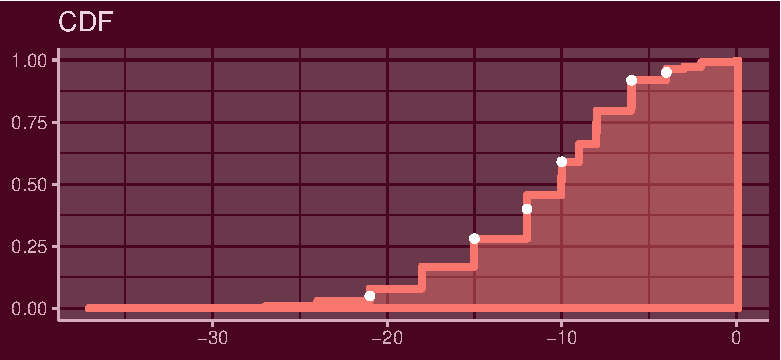
\includegraphics{sablica-hornik_files/figure-latex/unnamed-chunk-14-1} 
\caption{CDF plot of the \texttt{-DM} object with calculated quantiles annotated with white dots.}
\end{figure}
\end{Schunk}


Finally, since inverse transform sampling is not efficient for mixture
distributions, it can be replaced by first sampling according to the
weights \(w_{i}\) and then, conditionally on that, by drawing from the
selected component, similarly as in the \CRANpkg{actuar} package
\citep{actuar}. This approach is implemented in the corresponding method
of the \texttt{r()} function. This allows to draw from a mixture much
faster than the inverse quantile transform method and can also be reused
later for composite distributions. Besides the quantile function and 
other main functions for evaluation,
one can call other generic functions that are designed for the class
\textmd{\textsl{mixdist}}, e.g. \texttt{sudo\textunderscore support()}.

\begin{Schunk}
\begin{Sinput}
sudo_support(M)
\end{Sinput}
\begin{Soutput}
#> From   To 
#> -Inf  Inf
\end{Soutput}
\end{Schunk}

Since the mixture models are in fact distributions, one can perform
transformations of mixture random variables as well. It is easy to show
that a transformation of a mixture random variable is the same as if we
applied the same transformation to all of its components. In addition,
since the support of the components is a subset of the mixture's
support, if the framework allows to transform the mixture, then it does
the components as well. Now using the mixture we created, we can perform
a decreasing non-linear transformation. An example of \texttt{r()} and
\texttt{autoplot()} follows.

\begin{Schunk}
\begin{Sinput}
M_trans <- -2 * (M)^(1/3)
r(M_trans, 4)
\end{Sinput}
\begin{Soutput}
#> [1]  1.757693  2.247355  2.387137 -1.986538
\end{Soutput}
\end{Schunk}

\begin{Schunk}
\begin{Sinput}
autoplot(M_trans)
\end{Sinput}

\begin{figure}[h]
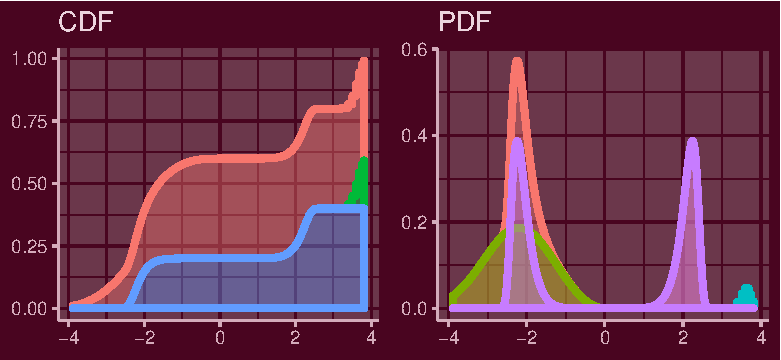
\includegraphics{sablica-hornik_files/figure-latex/unnamed-chunk-17-1} 
\caption{CDF (left) and PDF (right) plot of the \texttt{M\_trans} object.}
\end{figure}
\end{Schunk}



\hypertarget{composite-distributions}{%
\subsubsection{Composite distributions}\label{composite-distributions}}

Function \texttt{compdist()} creates composite distributions, which like
mixture distributions can be done in two ways. Either one can directly
use the objects or let the function create these objects by specifying
the sequence of names and a list of parameters. In the following
example, we will directly proceed with the first method where we define
some objects inside the \texttt{compdist()} call to create a composite
distribution. Besides these objects one needs to set the sequences of
weights and breakpoints. Additionally, one may determine for each
breakpoint to which partition should the breakpoint be included. This
can be set by the argument \code{break.spec} with values `R' or `L',
where `R' and `L' stand for right (i.e., include breakpoint to the
interval on the right of the breakpoint) and left (i.e., include to the
interval on the left), respectively. If this argument is not stated, the
algorithm will by default set all intervals to be left-closed, i.e.,
right-open. This can be nicely seen from the following example where a
linearly transformed Pareto distribution and a geometric distribution
are combined with a normal distribution into a composite model.

\begin{Schunk}
\begin{Sinput}
C <- compdist(-paretodist(1, 1), normdist(0, 2), geomdist(0.3) + 2, 
              weights = c(0.15, 0.7, 0.15), breakpoints = c(-3, 3),
              break.spec = c("L", "R"))
C
\end{Sinput}
\begin{Soutput}
#> Composite distribution with: 
#>  
#>   Trafo Distribution           Parameters Weight Truncation
#> 1  -X       Pareto   scale = 1, shape = 1   0.15  (-Inf,-3]
#> 2 none      Normal     mean = 0, sd = 2     0.70   (-3,3)  
#> 3 X + 2    Geometric      prob = 0.3        0.15   [3,Inf)
\end{Soutput}
\end{Schunk}

\noindent The argument \code{break.spec} is set to (``L'', ``R''), and
thus the breakpoint \(-3\) belongs to the first partition while the
second breakpoint is affiliated to the partition on the right. This can
be observed from the print of the distribution, more precisely from the
Truncation column, where the parentheses are printed according to this
argument.

The package also permits to use the same breakpoint twice. This
possibility allows to define a partition on a singleton, and hence to
create a mass of probability. If this feature is used, the
\code{break.spec} needs to be specified with ``R'' and ``L'', for the
first and second identical breakpoint, respectively, or not set at all.
If the \code{break.spec} is not used, the source code will change
\code{break.spec} such that this single point with probability mass is a
closed set. This feature can become particularly useful when the user
wants to create a distribution that is, for example, absolutely
continuous on both the negative and positive reals and has positive mass
at zero.

\begin{Schunk}
\begin{Sinput}
C2 <- compdist(-expdist(2), poisdist(), expdist(2),
               weights = c(0.25, 0.5, 0.25), breakpoints = c(0, 0))
C2
\end{Sinput}
\begin{Soutput}
#> Composite distribution with: 
#>  
#>   Trafo Distribution Parameters Weight Truncation
#> 1  -X    Exponential  rate = 2    0.25   (-Inf,0)
#> 2 none     Poisson   lambda = 1   0.50    [0,0]  
#> 3 none   Exponential  rate = 2    0.25   (0,Inf)
\end{Soutput}
\end{Schunk}

\noindent Note that the distribution assigned to this singleton has to
be a discrete distribution with support on that point, otherwise the
interval will have zero probability.

As for any distribution, the framework offers many methods that can be
used to obtain additional information or evaluate the composite
distribution. One can extract the parameters, weights, or the support in
the same manner as with mixture distributions. In addition, calling
\texttt{breakpoints()} extracts the splicing points. Finally, there are
methods for \texttt{plot()} and \texttt{autoplot()} where the components
are shown by default, which again can be turned off using the
\code{only\textunderscore mix = TRUE} argument.

\begin{Schunk}
\begin{Sinput}
par(mai = c(0.4, 0.4, 0.2, 0.2))
plot(C, xlim1 = c(-15, 15), ylab1 = "", cex.axis = 0.75, mtext_cex = 0.75)
\end{Sinput}

\begin{figure}[h]
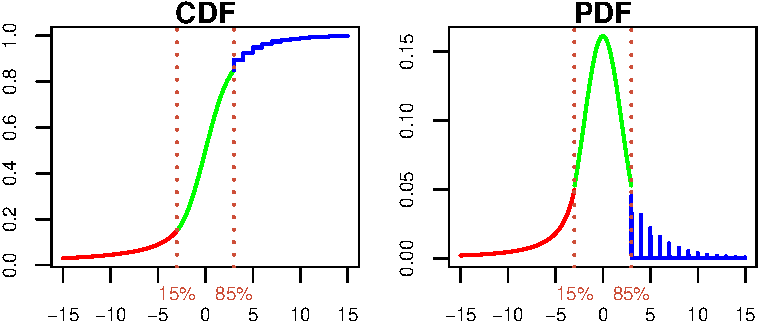
\includegraphics{sablica-hornik_files/figure-latex/unnamed-chunk-20-1} 
\caption{CDF (left) and PDF (right) plot of the \texttt{C} object using \texttt{plot()}.}
\end{figure}
\end{Schunk}

\begin{Schunk}
\begin{Sinput}
autoplot(C2, text_ylim = 0.01)
\end{Sinput}

\begin{figure}[h]
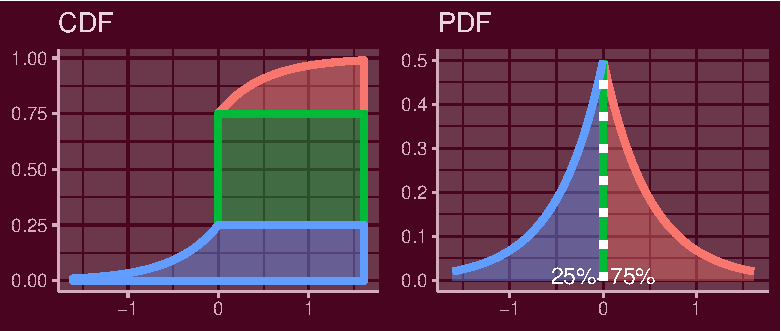
\includegraphics{sablica-hornik_files/figure-latex/unnamed-chunk-21-1} 
\caption{CDF (left) and PDF (right) plot of the \texttt{C2} object using \texttt{autoplot()}.}
\end{figure}
\end{Schunk}

Analogously to the mixture distributions, the framework also supports
the transformations of composite random variables. Thus, using the
composite distribution we defined, we propose an example of a linear
transformation.

\begin{Schunk}
\begin{Sinput}
C_trans <- -0.5 * (C + 7)
\end{Sinput}
\end{Schunk}

Even with such a distribution, the user still can evaluate all functions
``of interest''. To support this, an example follows where the function
\texttt{q()} and \texttt{r()} are used, and the functions \texttt{p()}
and \texttt{d()} are represented graphically using the
\texttt{autoplot()} method.

\begin{Schunk}
\begin{Sinput}
q(C_trans, c(0.075, 0.5, 0.7, 0.9))
\end{Sinput}
\begin{Soutput}
#> [1] -5.500000 -3.500000 -2.833235 -1.250000
\end{Soutput}
\begin{Sinput}
r(C_trans, 4)
\end{Sinput}
\begin{Soutput}
#> [1] -4.635072 -3.161199 -5.500000 -4.817573
\end{Soutput}
\end{Schunk}

\begin{Schunk}
\begin{Sinput}
autoplot(C_trans, xlim1 = c(-10,5))
\end{Sinput}

\begin{figure}[h]
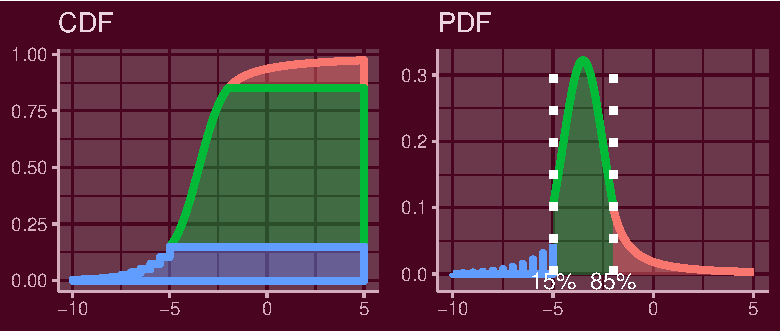
\includegraphics{sablica-hornik_files/figure-latex/unnamed-chunk-24-1} 
\caption{CDF (left) and PDF (right) plot of the \texttt{C\_trans} object using \texttt{autoplot()}.}
\end{figure}
\end{Schunk}

\hypertarget{combining-mixture-and-composite-distributions}{%
\subsection{Combining mixture and composite
distributions}\label{combining-mixture-and-composite-distributions}}

A significant advantage of object oriented programming is that the
dispatching mechanism automatically knows how to treat a given object.
This allows to combine mixture and composite models into more
complicated mixtures and composite distributions. Therefore, we can take
the transformed mixture and the transformed composite distribution that
we created in the last chapter to compose a composite distribution with
these distributions as components. What is more, we can perform further
transformations of such a distribution.

\begin{Schunk}
\begin{Sinput}
C3 <- compdist(M_trans - 3, C_trans, weights = c(0.5, 0.5), breakpoints = -4.5)
C3_trans <- -2 * C3 + 2
\end{Sinput}
\end{Schunk}

Thus, the object \texttt{C3\textunderscore trans} is a transformed
composite distribution that contains a transformed mixture and a
transformed composite distribution, from which both additionally contain
many transformed and untransformed distributions. Even in such complex
models, the user may evaluate the most complicated functions like
\texttt{plim()} and \texttt{qlim()}. The functions \texttt{d()} and
\texttt{p()} can be again best represented graphically, where both
distributions can easily be recognized from previous chapters.



\begin{Schunk}
\begin{Sinput}
autoplot(C3_trans, xlim1 = c(0,20), text_ylim = 0.01, grey = TRUE)
\end{Sinput}

\begin{figure}[h]
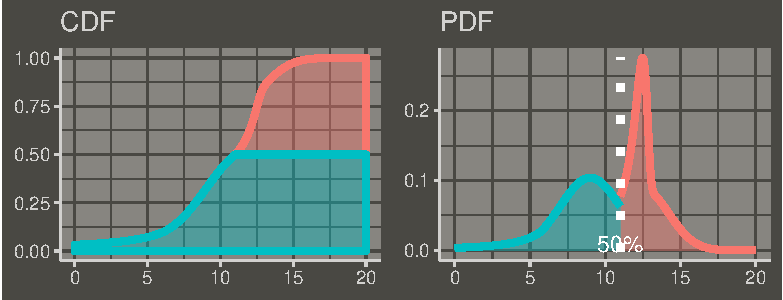
\includegraphics{sablica-hornik_files/figure-latex/unnamed-chunk-27-1} 
\caption{CDF (left) and PDF (right) plot of the \texttt{C3\_trans} object.}
\end{figure}
\end{Schunk}

\begin{Schunk}
\begin{Sinput}
plim(C3_trans, c(6, 10, 12))
\end{Sinput}
\begin{Soutput}
#> [1] 0.09667553 0.42195189 0.62458021
\end{Soutput}
\begin{Sinput}
qlim(C3_trans, c(0.3, 0.5, 0.7))
\end{Sinput}
\begin{Soutput}
#> [1]  8.785363 11.000000 12.327907
\end{Soutput}
\end{Schunk}

As the \texttt{print()} output for such a hierarchical distribution does
not contain lot of information, one can alternatively use
\texttt{summary()} for which the package provides methods, which are
particularly useful for the hierarchical distributions. The printed
result of this call consists of all the necessary information, and much
more as well. Nevertheless, since the result of \texttt{summary()} on
the \texttt{C3\_trans} object is two pages long, the demonstration is
left to the reader.

To finish this chapter and to show that the user may go even further, we
present an example where we combine the last object with another
distribution from this chapter into a mixture distribution. The
distribution is directly plotted using autoplot().

\begin{Schunk}
\begin{Sinput}
autoplot(mixdist( C3_trans, C2 + 5, weights = c(0.7, 0.3)), xlim1 = c(0, 15))
\end{Sinput}

\begin{figure}[h]
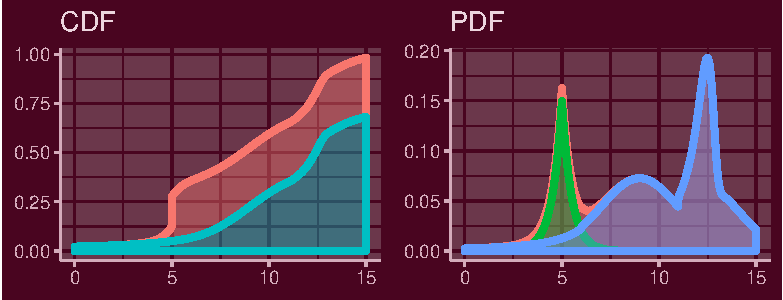
\includegraphics{sablica-hornik_files/figure-latex/unnamed-chunk-28-1} 
\caption{CDF (left) and PDF (right) plot of the mixture distribution with components \texttt{C3\_trans} and \texttt{C2 + 5}.}
\end{figure}
\end{Schunk}

\hypertarget{data-modeling}{%
\section{Data modeling}\label{data-modeling}}

While the previous chapters were aimed at showing the ``muscles'' (i.e.,
generality) of the framework, in this last chapter we will focus on
examples using real data. In particular, we will present a simple
fitting for two specific composite distributions.

As motivated in the introduction, the models in financial and actuarial
mathematics suggest employing distributions which can capture the wide
variety of behaviors in tails while still following the normal
distribution in the center. In the two-tailed case, this suggests to use
a three components composite distribution, where the first and third
component will be used to model the extreme cases, i.e., the tails, and
the second component will try to catch the center of the empirical
distribution.

The first model offered by \pkg{mistr} is the Pareto-Normal-Pareto (PNP)
model. This means that a \(-X\) transformation of a Pareto random
variable will be used for the left tail, normal distribution for the
center and again Pareto for the right tail. From this it follows that
the PDF of the model can be written as: \[
f(x)= \left\{\begin{matrix}
w_{1}\frac{f_{-P}(x)}{F_{-P}(\beta_{1} )} & \text{   if}& -\infty< x< \beta_{1},\\
w_{2}\frac{f_{N}(x)}{F_{N}(\beta_{2} )-F_{N}(\beta_{1} )} & \text{ if}& \beta_{1}\leq x<\beta_{2},   \\
w_{3}\frac{f_{P}(x)}{1-F_{P}(\beta_{2} )} & \text{  if} &\beta_{2}  \leq x< \infty,
\end{matrix}\right.
\] where \(f_{P}(x)=f_{-P}(-x)\) and \(F_{P}(x)=1-(K/x)^\alpha\) are the
density and distribution function of a Pareto distribution with
\(F_{-P}(x)=1-F_{P}(-x)\). \(f_{N}(x)\) and \(F_{N}(x)\) are the PDF and
CDF of the normal distribution, respectively.

If we follow the properties of a Pareto distribution, the conditional
probability distribution of a Pareto-distributed random variable, given
that the event is greater than or equal to \(\gamma>K\), is again a
Pareto distribution with parameters \(\gamma\) and \(\alpha\). This
means that the conditional distribution
\(f_{P}(x|K,\alpha)/(1-F_{P}(\beta_{2} |K,\alpha))=f_{P}(x|\beta_{2},\alpha)\)
if \(\beta_{2}>K\). On the other hand, if \(\beta_{2}<K\) the
distribution cannot be continuous as the support of a Pareto
distribution starts at \(K\). The same can be shown for the transformed
distribution and hence we can rewrite the PDF as \[
f(x)= \left\{\begin{matrix}
w_{1}f_{-P}(x|-\beta_{1},\alpha_{1}) & \text{  if}& -\infty< x< \beta_{1},\\
w_{2}\frac{f_{N}(x|\mu,\sigma)}{F_{N}(\beta_{2}|\mu,\sigma)-F_{N}(\beta_{1}|\mu,\sigma )} & \text{ if}& \beta_{1}\leq x<\beta_{2},   \\
w_{3}f_{P}(x|\beta_{2},\alpha_{2}) & \text{  if} &\beta_{2}  \leq x< \infty,
\end{matrix}\right. \quad  
\text{where} \quad  \begin{matrix}
\beta_{1}<0<\beta_{2},\\
\alpha_{1},\alpha_{2}> 0.
\end{matrix}
\]

The condition \(\beta_{1}<0<\beta_{2}\) follows from the fact that the
scale parameter has to be positive. Thus, such a model can be fully used
only with demeaned data sample or with data with a mean close to zero.
This is of course not a problem for stock returns, which are the aim of
this chapter. What is more, one can show that the density is continuous
if for the shape parameters it holds that \[
\alpha_{1} =-\beta_{1} \frac{w_{2}f_{N}(\beta_{1}|\mu,\sigma)}{w_{1}\left (F_{N}(\beta_{2}|\mu,\sigma)-F_{N}(\beta_{1}|\mu,\sigma )  \right )},
\] \[
 \quad \alpha_{2} =\beta_{2} \frac{w_{2}f_{N}(\beta_{2}|\mu,\sigma)}{w_{3}\left (F_{N}(\beta_{2}|\mu,\sigma)-F_{N}(\beta_{1}|\mu,\sigma )  \right )}.
 \] This condition is not only natural when modelling the real data, it additionally solves the possible instability effects at estimation once observations come to lie close to breakpoints. Due to the fact that a composite distribution can be represented as
a mixture of truncated distributions that are truncated to a disjoint
support, the weight of each component can be estimated as the proportion
of points that correspond to each of the truncated regions. Obviously,
this condition ensures that the empirical and estimated CDF match on
each of the breakpoints. Thus, conditionally on the fact that the
breakpoints are known, similarly as in \cite{Erlang}, the weights can be computed as \[
w_{1}=\frac{\sum_{i=1}^{n}1_{\{x_{i}< \beta_{1}\}}}{n}  \text{, }  w_{2}=\frac{\sum_{i=1}^{n}1_{\{\beta_{1}\leq x_{i}<\beta_{2}\}}}{n}, 
w_{3}=\frac{\sum_{i=1}^{n}1_{\{\beta_{2}\leq x_{i}\}}}{n},
\] where \(1_{\{\cdot\}}\) is the indicator function and \(x_{i}\) is
the i-th data value. These conditions decrease the number of parameters
from 11 to 4 and imply the density function of the form: \[
f(x|\beta_{1},\beta_{2},\mu,\sigma).
\]

This model is offered by the function \texttt{PNP\textunderscore fit()}
which takes the data and a named vector of starting values with names
\code{break1}, \code{break2}, \code{mean}, and \code{sd} and returns a
list of class \textmd{\textsl{comp\textunderscore fit}}. Other arguments
are passed to the optimizer which then maximizes the likelihood of the
above specified model. The optimization is handled by the
\texttt{mle2()} function from \CRANpkg{bbmle} package \citep{mle}. To
demonstrate this, we will take the same data we used in the introduction
to fit a PNP model with the default starting values.

\begin{Schunk}
\begin{Sinput}
PNP_model <- PNP_fit(stocks$SAP)

PNP_model
\end{Sinput}
\begin{Soutput}
#> Fitted composite Pareto-Normal-Pareto distribution: 
#> 
#> Breakpoints: -0.019304 0.020518 
#> Weights: 0.092443 0.82135 0.086207 
#> 
#> Parameters: 
#>   scale1   shape1     mean       sd   scale2   shape2 
#> 0.019304 1.773598 0.000961 0.012950 0.020518 2.198590 
#> 
#> Log-likelihood: 7400.117,  Average log-likelihood: 2.7146
\end{Soutput}
\end{Schunk}

If the fitted object is printed, the function prints all the parameters
together with the log-likelihood that was achieved by the optimization.
In addition, the average log-likelihood is printed, which is just the
log-likelihood divided by the size of the data set. The user can extract
parameters using \texttt{parameters()}, weights using
\texttt{weights()}, and breakpoints using \texttt{breakpoints()}. The
\texttt{distribution()} function can be used to extract the distribution
with fitted parameters that can be used for evaluation.

Finally, again \texttt{plot()} and \texttt{autoplot()} methods are
offered, which give a Q-Q plot of the fitted distribution and the data,
and the CDF and PDF plot of the fitted distribution, which overlap with
the empirical CDF and PDF of the data set. Again, the \code{which}
argument can extract the proposed plots separately (i.e.,
\code{which = "pdf"}). Other arguments are passed to the the plot calls.

\begin{Schunk}
\begin{Sinput}
plot(PNP_model, ylab1 = "", ylab2 = "")
\end{Sinput}

\begin{figure}[h]
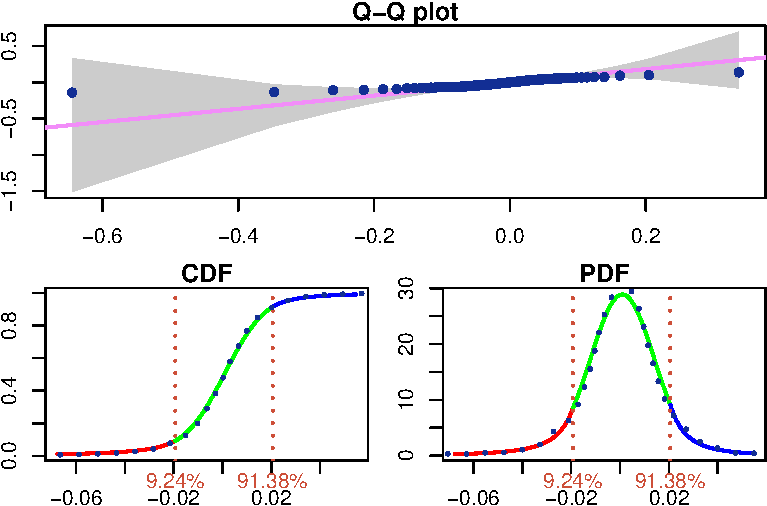
\includegraphics{sablica-hornik_files/figure-latex/unnamed-chunk-30-1} 
\caption{Q-Q (up), CDF (bottom left) and PDF (bottom right) plot of the fitted PNP model overlapped with empirical results indicated by blue dots using \texttt{plot()}.}
\end{figure}
\end{Schunk}

\noindent The plots indicate an overall nice fit where all quantiles are
in the confidence bound.

The second model offered is a similar distribution to the previous one,
except we will replace the Pareto distributions by the generalized
Pareto distributions (GPD) \[F_{GPD}(x)=\left\{\begin{matrix}
1-\left ( 1+\xi \frac{x-\theta }{\gamma} \right )^{-1/\xi  }  &  \text{if } \xi\neq0,\\
 1-\exp\left (  -\frac{x-\theta }{\gamma}\right )&  \text{if } \xi=0.
\end{matrix}\right.\] This means that the PDF of this model can be
written as: \[
f(x)= \left\{\begin{matrix}
w_{1}\frac{f_{-GPD}(x)}{F_{-GPD}(\beta_{1} )} & \text{ if}& -\infty< x< \beta_{1},\\
w_{2}\frac{f_{N}(x)}{F_{N}(\beta_{2} )-F_{N}(\beta_{1} )} & \text{ if}& \beta_{1}\leq x<\beta_{2},   \\
w_{3}\frac{f_{GPD}(x)}{1-F_{GPD}(\beta_{2} )} & \text{  if} &\beta_{2}  \leq x< \infty.
\end{matrix}\right.
\]

The same way as in the PNP model, the scale parameters can be eliminated
by the continuity conditions, weights by the above mentioned condition
and in addition, under current settings and the continuity conditions,
the value of the conditional GPD distribution depends on the location
parameter only through the conditions \(-\beta_{1}\geq\theta_{1}\) and
\(\beta_{2}\geq\theta_{2}\). This suggests to choose without any loss in
the model \(-\beta_{1}=\theta_{1}\) and \(\beta_{2}=\theta_{2}\). This
PDF is then fully characterized by \[
 f(x|\beta_{1},\beta_{2},\mu,\sigma,\xi_{1},\xi_{2}),
\] where the only restriction on the parameters is
\(-\infty<\beta_{1}<\beta_{2}<\infty\).

These conditions decrease the number of parameters from 13 to 6. What is
more, the function \texttt{GNG\textunderscore fit()} contains the
argument \code{break\textunderscore fix}, which fixes the breakpoints
from the vector of starting values, and so decreases the number of
parameters to 4 if \code{TRUE} is assigned. In this case, the
breakpoints are fixed and weights are computed before the optimization.
The function \texttt{GNG\textunderscore fit()} takes the data, the named
vector of starting values with names \code{break1}, \code{break2},
\code{mean}, \code{sd}, \code{shape1} and \code{shape2}, the
\code{break\_fix} argument and the argument \code{midd}, which is by
default set to be equal to the mean of the data. The \code{midd} value
is used to split \(\mathbb{R}\) into two sub-intervals and then the
first breakpoint is optimized on the left of the \code{midd} value and
the second breakpoint on the right.

The function returns a list of class
\textmd{\textsl{comp\textunderscore fit}}. The results can be then
extracted, printed or visualized in the same way as the results of
\texttt{PNP\textunderscore fit()}.

\begin{Schunk}
\begin{Sinput}
GNG_model <- GNG_fit(stocks$SAP)

GNG_model
\end{Sinput}
\begin{Soutput}
#> Fitted composite GPD-Normal-GPD distribution: 
#> 
#> Breakpoints: -0.019414 0.019353 
#> Weights: 0.091343 0.812546 0.096112 
#> 
#> Parameters: 
#>     loc1   scale1   shape1     mean       sd     loc2   scale2   shape2 
#> 0.019414 0.013439 0.150141 0.000907 0.011696 0.019353 0.010842 0.096832 
#> 
#> Log-likelihood: 7423.245,  Average log-likelihood: 2.7231
\end{Soutput}
\end{Schunk}

\begin{Schunk}
\begin{Sinput}
autoplot(GNG_model)
\end{Sinput}

\begin{figure}[h]
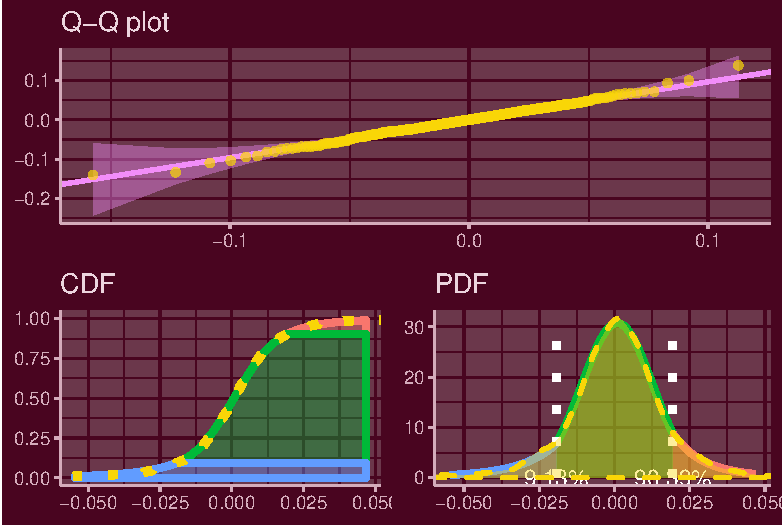
\includegraphics{sablica-hornik_files/figure-latex/unnamed-chunk-32-1} 
\caption{Q-Q (up), CDF (bottom left) and PDF (bottom right) plot of the fitted GNG model overlapped with empirical results indicated by yellow dots and dashes using \texttt{autoplot()}.}
\end{figure}
\end{Schunk}

The log-likelihood has increased to 7423.2 with the average of 2.723 per
data-point. In this model, the generalized Pareto distribution explains
the first 9.1\% from the left tail and the last 9.6\% from the right
tail. Since the GPD generalizes the Pareto distribution, the higher
likelihood is a reasonable result. Moreover, the QQ-plot suggests an
almost perfect fit.

The result of these estimations is a proper continuous parametric set-up
that describes the distribution of the data. What is more, the
distribution has been fitted as a whole with respect to the continuity
conditions. This means that the tails take into account the whole
distribution, which allows to calculate the risk measures with an even
higher precision as when only the tails are modeled.

\hypertarget{risk-measures}{%
\subsection{Risk measures}\label{risk-measures}}

Package \pkg{mistr} provides a function \texttt{risk()} which can be
used for rapid calculations of point estimates of prescribed quantiles,
expected shortfalls and expectiles (in the following table denoted as
VaR, ES and Exp, respectively). For more details on these measures see
\citet{McNeil:2015:QRM:2811305}. As input parameters this function needs
the output of the function \texttt{PNP\textunderscore fit()} or
\texttt{GNG\textunderscore fit()} and a vector of the desired levels. As
an example we illustrate this function on our fitted object.

\begin{Schunk}
\begin{Sinput}
risk(GNG_model, c(0.02, 0.05, 0.07, 0.1, 0.2, 0.3))
\end{Sinput}
\begin{Soutput}
#>   level         VaR         ES         Exp
#> 1  0.02 0.042341368 0.06220519 0.032240507
#> 2  0.05 0.027889909 0.04520065 0.021949976
#> 3  0.07 0.023062791 0.03952074 0.018526202
#> 4  0.10 0.018245509 0.03380624 0.015091608
#> 5  0.20 0.010642738 0.02386181 0.008851640
#> 6  0.30 0.006167236 0.01867190 0.005168659
\end{Soutput}
\end{Schunk}

\noindent These results can be also visualized if arguments \code{plot}
or \code{ggplot} are set to \code{TRUE}.

\hypertarget{summary}{%
\section{Summary}\label{summary}}

We introduced a new extensible framework for mixture and composite
distributions in R via the \pkg{mistr} package. It offers creation and
manipulation of simple distributions which can be combined into more
complicated distributions to offer more generality in the current data
modeling. Furthermore, the framework provides multiple methods
specifically designed to describe and visualize the distributions or
functions capable of fitting the two pre-defined composite distributions
introduced in the last chapter.

The package is additionally equipped with the possibility to extend the
current list of known distributions and monotone transformations by letting the
user add these in a very simple way. This procedure is documented in
detail in the
\href{https://cran.r-project.org/web/packages/mistr/vignettes/mistr-extensions.pdf}{Extensions vignette}.
Finally, we will keep adding multiple extensions and distributions to
extend the generality even more.


\bibliography{sablica-hornik}


\address{%
Lukas Sablica\\
Institute for Statistics and Mathematics\\
Vienna University of Economics and Business\\
Austria\\
\url{https://www.wu.ac.at/en/statmath}\\
ORCiD: 0000-0001-9166-4563\\
}
\href{mailto:lsablica@wu.ac.at}{\nolinkurl{lsablica@wu.ac.at}}

\address{%
Kurt Hornik\\
Institute for Statistics and Mathematics\\
Vienna University of Economics and Business\\
Austria\\
\url{https://www.wu.ac.at/en/statmath}\\
ORCiD: 0000-0003-4198-9911\\
}
\href{mailto:Kurt.Hornik@wu.ac.at}{\nolinkurl{Kurt.Hornik@wu.ac.at}}

